\section{向量场在曲面上的积分}

\begin{problem}{第二型曲面积分}{Surface-Integrals-of-Second-Kind}
    计算下列第二型曲面积分：
    \begin{enumerate}
        \item $\iint_{S} (x + y^2 + z) \d x \d y$，其中 $S$ 为椭球面 $\frac{x^2}{a^2} + \frac{y^2}{b^2} + \frac{z^2}{c^2} = 1$ 的外侧；
        \item $\iint_{S} x y z \d x \d y$，$S$ 是柱面 $x^2 + z^2 = R^2$ 在 $x \ge 0$、 $y \ge 0$ 两卦限内被平面 $y = 0$ 及 $y = h$ 所截下部分的外侧；
        \item $\iint_{S} x y^2 z^2 \d y \d z$，$S$ 为球面 $x^2 + y^2 + z^2 = R^2$ 的 $x \le 0$ 的一半远离球心一侧；
        \item $\iint_{S} y z \d z \d x$，$S$ 为球面 $x^2 + y^2 + z^2 = 1$ 的上半部分 ($z \ge 0$) 并取外侧；
        \item $\iint_{S} x^2 \d y \d z + y^2 \d z \d x + z^2 \d x \d y$，$S$ 为平面 $x + y + z = 1$ 在第一卦限的部分，远离原点的一侧；
        \item $\iint_{S} (y - z) \d y \d z + (z - x) \d z \d x + (x - y) \d x \d y$，$S$ 是圆锥面 $x^2 + y^2 = z^2$ ($0 \le z \le 1$) 的下侧；
        \item $\iint_{S} x z^2 \d y \d z + x^2 y \d z \d x + y^2 z \d x \d y$，$S$ 是通过上半球面 $z = \sqrt{a^2 - x^2 - y^2}$ 的上侧；
        \item $\iint_{S} f(x) \d y \d z + g(y) \d z \d x + h(z) \d x \d y$，其中 $f(x)$、$g(y)$、$h(z)$ 为连续函数，$S$ 为直角平行六面体 $0 \le x \le a$、$0 \le y \le b$、$0 \le z \le c$ 的外侧．
    \end{enumerate}
\end{problem}

\begin{solution}
    \ansitem{1}

    设 $\Omega$ 为椭球体 $\frac{x^2}{a^2} + \frac{y^2}{b^2} + \frac{z^2}{c^2} \le 1$，其体积为 $V = \frac{4}{3} \uppi a b c$．因为曲面 $S$ 为 $\Omega$ 的外侧，由高斯公式可得：
    \begin{equation}
        \label{eq:ellipsoid-1}
        \iint_{S} (x + y^2 + z) \d x \d y = \iiint_{\Omega} \frac{\partial}{\partial z} (x + y^2 + z) \d V = \iiint_{\Omega} 1 \d V.
    \end{equation}
    由此计算可得：
    \begin{equation}
        \label{eq:ellipsoid-2}
        \iint_{S} (x + y^2 + z) \d x \d y = \boxed{\frac{4}{3} \uppi a b c}.
    \end{equation}

    \ansitem{2}

    由于 $S$ 是圆柱面 $x^2 + z^2 = R^2$ 在 $x \ge 0$ 且 $0 \le y \le h$ 的外侧，可将 $S$ 分为上半部分 $S_1$（$z \ge 0$）和下半部分 $S_2$（$z < 0$）．
    上半部分 $S_1$ 的方程为 $z = \sqrt{R^2 - x^2}$，取外侧朝上，向 $xOy$ 平面投影区域为 $D_{xy} = \{ (x,y) \mid 0 \le x \le R, 0 \le y \le h \}$，转换二重积分符号为正；下半部分 $S_2$ 的方程为 $z = -\sqrt{R^2 - x^2}$，取外侧朝下，投影区域同样为 $D_{xy}$，转换二重积分符号为负．

    由此可得：
    \begin{equation}
        \label{eq:cylinder-1}
        \begin{aligned}
            \iint_{S} x y z \d x \d y & = \iint_{S_1} x y z \d x \d y + \iint_{S_2} x y z \d x \d y                                                         \\
                                      & = \iint_{D_{xy}} x y \sqrt{R^2 - x^2} \d x \d y + \iint_{D_{xy}} x y \left( -\sqrt{R^2 - x^2} \right) (- \d x \d y) \\
                                      & = 2 \iint_{D_{xy}} x y \sqrt{R^2 - x^2} \d x \d y.
        \end{aligned}
    \end{equation}
    计算二重积分可得：
    \begin{equation}
        \label{eq:cylinder-2}
        \begin{aligned}
            2 \iint_{D_{xy}} x y \sqrt{R^2 - x^2} \d x \d y & = 2 \left( \int_0^R x \sqrt{R^2 - x^2} \d x \right) \left( \int_0^h y \d y \right)                     \\
                                                            & = 2 \left[ -\frac{1}{3} (R^2 - x^2)^{\frac{3}{2}} \right]_0^R \cdot \left[ \frac{1}{2} y^2 \right]_0^h \\
                                                            & = 2 \left( \frac{1}{3} R^3 \right) \left( \frac{1}{2} h^2 \right).
        \end{aligned}
    \end{equation}
    因此，最终积分为：
    \begin{equation}
        \label{eq:cylinder-3}
        \iint_{S} x y z \d x \d y = \boxed{\frac{1}{3} R^3 h^2}.
    \end{equation}

    \ansitem{3}

    补面 $S_0: x = 0$（其中 $y^2 + z^2 \le R^2$），取右侧，其法向量为 $(1, 0, 0)$．
    此时半球面 $S$ 与平面 $S_0$ 共同围成闭区域 $\Omega = \{ (x, y, z) \mid x^2 + y^2 + z^2 \le R^2, x \le 0 \}$ 的外侧．
    在 $S_0$ 上，因为 $x = 0$，故被积函数为 $0$，即 $\iint_{S_0} x y^2 z^2 \d y \d z = 0$．由高斯公式可得：
    \begin{equation}
        \label{eq:hemisphere-left-1}
        \iint_{S} x y^2 z^2 \d y \d z = \iint_{S + S_0} x y^2 z^2 \d y \d z = \iiint_{\Omega} \frac{\partial}{\partial x} (x y^2 z^2) \d V = \iiint_{\Omega} y^2 z^2 \d V.
    \end{equation}
    引入球面坐标，因为 $x \le 0$，所以 $\varphi \in \left[ \frac{\uppi}{2}, \uppi \right]$，$\theta \in [0, 2\uppi]$，$\rho \in [0, R]$：
    \begin{equation}
        \label{eq:hemisphere-left-2}
        \begin{aligned}
            \iiint_{\Omega} y^2 z^2 \d V & = \int_0^R \rho^6 \d \rho \int_{\frac{\uppi}{2}}^{\uppi} \sin^5 \varphi \d \varphi \int_0^{2\uppi} \cos^2 \theta \sin^2 \theta \d \theta              \\
                                         & = \frac{R^7}{7} \cdot \left( \int_0^{\frac{\uppi}{2}} \sin^5 t \d t \right) \cdot \left( \frac{1}{4} \int_0^{2\uppi} \sin^2 2\theta \d \theta \right) \\
                                         & = \frac{R^7}{7} \cdot \frac{8}{15} \cdot \frac{\uppi}{4}.
        \end{aligned}
    \end{equation}
    由此可得最终答案：
    \begin{equation}
        \label{eq:hemisphere-left-3}
        \iint_{S} x y^2 z^2 \d y \d z = \boxed{\frac{2 \uppi}{105} R^7}.
    \end{equation}

    \ansitem{4}

    补底面 $S_0: z = 0$（其中 $x^2 + y^2 \le 1$），取下侧，其指向向 $z$ 轴负方向．
    此时上半球面 $S$ 与底面 $S_0$ 共同围成闭区域 $\Omega = \{ (x, y, z) \mid x^2 + y^2 + z^2 \le 1, z \ge 0 \}$ 的外侧．
    在 $S_0$ 上，因为 $z = 0$，所以被积项为 $0$，即 $\iint_{S_0} y z \d z \d x = 0$．由高斯公式可得：
    \begin{equation}
        \label{eq:hemisphere-top-1}
        \iint_{S} y z \d z \d x = \iint_{S + S_0} y z \d z \d x = \iiint_{\Omega} \frac{\partial}{\partial y} (y z) \d V = \iiint_{\Omega} z \d V.
    \end{equation}
    利用柱面坐标进行计算：
    \begin{equation}
        \label{eq:hemisphere-top-2}
        \begin{aligned}
            \iiint_{\Omega} z \d V & = \iint_{x^2 + y^2 \le 1} \d x \d y \int_0^{\sqrt{1 - x^2 - y^2}} z \d z \\
                                   & = \frac{1}{2} \iint_{x^2 + y^2 \le 1} (1 - x^2 - y^2) \d x \d y          \\
                                   & = \frac{1}{2} \int_0^{2\uppi} \d \theta \int_0^1 (1 - r^2) r \d r        \\
                                   & = \uppi \left[ \frac{r^2}{2} - \frac{r^4}{4} \right]_0^1.
        \end{aligned}
    \end{equation}
    计算后可得最终答案：
    \begin{equation}
        \label{eq:hemisphere-top-3}
        \iint_{S} y z \d z \d x = \boxed{\frac{\uppi}{4}}.
    \end{equation}

    \ansitem{5}

    补三个平面区域 $S_1: x = 0$（在 $yOz$ 平面上）、$S_2: y = 0$（在 $zOx$ 平面上）、$S_3: z = 0$（在 $xOy$ 平面上），均取朝向原点的一侧，即外侧．
    这四个面共同包围了第一卦限内的四面体闭区域 $\Omega = \{ (x,y,z) \mid x \ge 0, y \ge 0, z \ge 0, x+y+z \le 1 \}$ 的外侧．
    在这三个补充面上，相应的坐标常数为 $0$，故其积分为 $0$．由高斯公式可得：
    \begin{equation}
        \label{eq:tetrahedron-1}
        \begin{aligned}
            \iint_{S} x^2 \d y \d z + y^2 \d z \d x + z^2 \d x \d y & = \iiint_{\Omega} \left( \frac{\partial(x^2)}{\partial x} + \frac{\partial(y^2)}{\partial y} + \frac{\partial(z^2)}{\partial z} \right) \d V \\
                                                                    & = 2 \iiint_{\Omega} (x + y + z) \d V.
        \end{aligned}
    \end{equation}
    根据对称性，$\iiint_{\Omega} x \d V = \iiint_{\Omega} y \d V = \iiint_{\Omega} z \d V$，因此有：
    \begin{equation}
        \label{eq:tetrahedron-2}
        2 \iiint_{\Omega} (x + y + z) \d V = 6 \iiint_{\Omega} z \d V.
    \end{equation}
    计算该三重积分：
    \begin{equation}
        \label{eq:tetrahedron-3}
        \begin{aligned}
            6 \iiint_{\Omega} z \d V & = 6 \int_0^1 z \d z \iint_{x+y \le 1-z} \d x \d y           \\
                                     & = 6 \int_0^1 z \cdot \frac{1}{2} (1 - z)^2 \d z             \\
                                     & = 3 \int_0^1 (z - 2z^2 + z^3) \d z                          \\
                                     & = 3 \left( \frac{1}{2} - \frac{2}{3} + \frac{1}{4} \right).
        \end{aligned}
    \end{equation}
    故得到最终结果：
    \begin{equation}
        \label{eq:tetrahedron-4}
        \iint_{S} x^2 \d y \d z + y^2 \d z \d x + z^2 \d x \d y = \boxed{\frac{1}{4}}.
    \end{equation}

    \ansitem{6}

    补顶盖面 $S_0: z = 1$（其中 $x^2 + y^2 \le 1$），取上侧，其法向量为 $(0, 0, 1)$．
    此时圆锥面 $S$ 与平面 $S_0$ 共同围成闭区域 $\Omega = \{ (x, y, z) \mid \sqrt{x^2 + y^2} \le z \le 1 \}$ 的外侧．由高斯公式可得：
    \begin{equation}
        \label{eq:cone-1}
        \begin{aligned}
             & \iint_{S + S_0} (y - z) \d y \d z + (z - x) \d z \d x + (x - y) \d x \d y                                                                    \\
             & = \iiint_{\Omega} \left[ \frac{\partial(y-z)}{\partial x} + \frac{\partial(z-x)}{\partial y} + \frac{\partial(x-y)}{\partial z} \right] \d V \\
             & = 0.
        \end{aligned}
    \end{equation}
    因此，得到 $\iint_{S} = - \iint_{S_0}$．
    在 $S_0$ 上，因为 $z = 1$ 为常数，故 $\d z = 0$；又因为取上侧，所以有：
    \begin{equation}
        \label{eq:cone-2}
        \iint_{S_0} (y - z) \d y \d z + (z - x) \d z \d x + (x - y) \d x \d y = \iint_{x^2+y^2 \le 1} (x - y) \d x \d y.
    \end{equation}
    根据积分区域的对称性及被积函数的奇偶性，该积分为 $0$．
    所以：
    \begin{equation}
        \label{eq:cone-3}
        \iint_{S} (y - z) \d y \d z + (z - x) \d z \d x + (x - y) \d x \d y = \boxed{0}.
    \end{equation}

    \ansitem{7}

    补底面 $S_0: z = 0$（其中 $x^2 + y^2 \le a^2$），取下侧，其指向向 $z$ 轴负方向．
    此时上半球面 $S$ 与底面 $S_0$ 共同围成闭区域 $\Omega = \{ (x, y, z) \mid x^2 + y^2 + z^2 \le a^2, z \ge 0 \}$ 的外侧．
    在 $S_0$ 上，因为 $z = 0$ 且 $\d z = 0$，所以其曲面积分为 $0$．由高斯公式可得：
    \begin{equation}
        \label{eq:ball-half-1}
        \begin{aligned}
            \iint_{S} x z^2 \d y \d z + x^2 y \d z \d x + y^2 z \d x \d y & = \iiint_{\Omega} \left( \frac{\partial(x z^2)}{\partial x} + \frac{\partial(x^2 y)}{\partial y} + \frac{\partial(y^2 z)}{\partial z} \right) \d V \\
                                                                          & = \iiint_{\Omega} (x^2 + y^2 + z^2) \d V.
        \end{aligned}
    \end{equation}
    引入球面坐标进行计算，其中 $\rho \in [0, a]$，$\varphi \in \left[ 0, \frac{\uppi}{2} \right]$，$\theta \in [0, 2\uppi]$：
    \begin{equation}
        \label{eq:ball-half-2}
        \begin{aligned}
            \iiint_{\Omega} (x^2 + y^2 + z^2) \d V & = \int_0^{2\uppi} \d \theta \int_0^{\frac{\uppi}{2}} \sin \varphi \d \varphi \int_0^a \rho^4 \d \rho \\
                                                   & = 2 \uppi \cdot 1 \cdot \frac{a^5}{5}.
        \end{aligned}
    \end{equation}
    因此，最终答案为：
    \begin{equation}
        \label{eq:ball-half-3}
        \iint_{S} x z^2 \d y \d z + x^2 y \d z \d x + y^2 z \d x \d y = \boxed{\frac{2}{5} \uppi a^5}.
    \end{equation}

    \ansitem{8}

    设 $S$ 的六个面分别为：$S_{x=a}$（前侧，向外）、$S_{x=0}$（后侧，向外）、$S_{y=b}$（右侧，向外）、$S_{y=0}$（左侧，向外）、$S_{z=c}$（顶侧，向外）、$S_{z=0}$（底侧，向外）．
    我们在各个面上分别计算曲面积分：
    对于 $S_{x=a}$，外侧法向量为 $(1, 0, 0)$，$\d x = 0$；对于 $S_{x=0}$，外侧法向量为 $(-1, 0, 0)$，$\d x = 0$．于是两面贡献的积分为：
    \begin{equation}
        \label{eq:box-1}
        \iint_{S_{x=a} + S_{x=0}} f(x) \d y \d z = \int_0^b \d y \int_0^c [f(a) - f(0)] \d z = [f(a) - f(0)] b c.
    \end{equation}
    同理，对于另外两对平行面有：
    \begin{equation}
        \label{eq:box-2}
        \iint_{S_{y=b} + S_{y=0}} g(y) \d z \d x = [g(b) - g(0)] a c,
    \end{equation}
    \begin{equation}
        \label{eq:box-3}
        \iint_{S_{z=c} + S_{z=0}} h(z) \d x \d y = [h(c) - h(0)] a b.
    \end{equation}
    将所有六个面的结果相加，即得最终答案：
    \begin{equation}
        \label{eq:box-4}
        \begin{aligned}
             & \iint_{S} f(x) \d y \d z + g(y) \d z \d x + h(z) \d x \d y           \\
             & = \boxed{[f(a) - f(0)] b c + [g(b) - g(0)] a c + [h(c) - h(0)] a b}.
        \end{aligned}
    \end{equation}
\end{solution}

\begin{problem}{高斯公式与通量计算}{Gauss-Theorem-Flux}
    求场 $\symbfit{v} = (x^3 - yz)\symbfit{i} - 2x^2y\symbfit{j} + z\symbfit{k}$ 通过长方体 $0 \le x \le a$、$0 \le y \le b$、$0 \le z \le c$ 的外侧表面 $S$ 的通量．
\end{problem}

\begin{solution}
    \begin{center}
        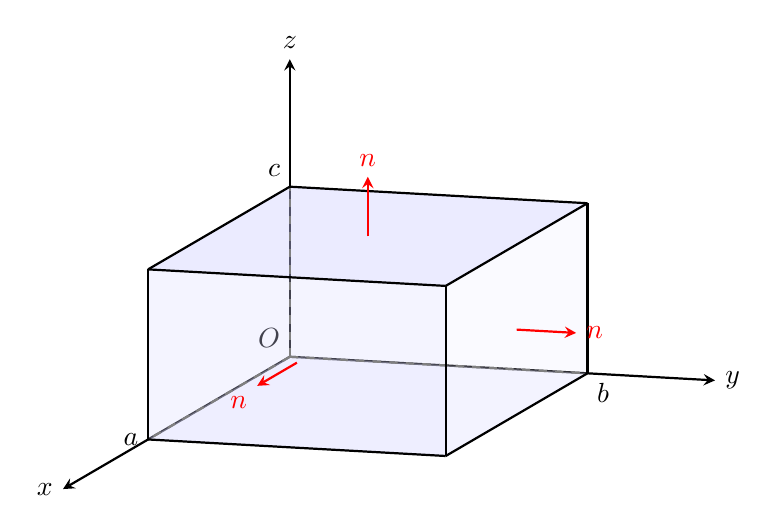
\begin{tikzpicture}[x={(-0.6cm,-0.35cm)}, y={(0.9cm,-0.05cm)}, z={(0cm,0.9cm)}, >=stealth, scale=1.2]
            % 坐标轴
            \draw[->, thick] (0,0,0) -- (4,0,0) node[left] {$x$};
            \draw[->, thick] (0,0,0) -- (0,5,0) node[right] {$y$};
            \draw[->, thick] (0,0,0) -- (0,0,3.5) node[above] {$z$};
            \node[anchor=south east] at (0,0,0) {$O$};

            % 长方体参数
            \def\a{2.5}
            \def\b{3.5}
            \def\c{2.0}

            % 绘制面（半透明填充以增强立体感）
            \fill[blue!10, opacity=0.3] (\a,0,0) -- (\a,\b,0) -- (0,\b,0) -- (0,0,0) -- cycle;
            \fill[blue!20, opacity=0.4] (0,0,\c) -- (\a,0,\c) -- (\a,\b,\c) -- (0,\b,\c) -- cycle;
            \fill[blue!15, opacity=0.3] (\a,0,0) -- (\a,\b,0) -- (\a,\b,\c) -- (\a,0,\c) -- cycle;
            \fill[blue!10, opacity=0.2] (0,\b,0) -- (\a,\b,0) -- (\a,\b,\c) -- (0,\b,\c) -- cycle;

            % 绘制看不见的虚线边
            \draw[dashed, thick, gray] (0,0,0) -- (\a,0,0);
            \draw[dashed, thick, gray] (0,0,0) -- (0,\b,0);
            \draw[dashed, thick, gray] (0,0,0) -- (0,0,\c);

            % 绘制可见的实线边
            \draw[thick] (\a,0,0) -- (\a,\b,0);
            \draw[thick] (0,\b,0) -- (\a,\b,0);
            \draw[thick] (\a,0,0) -- (\a,0,\c);
            \draw[thick] (0,\b,0) -- (0,\b,\c);
            \draw[thick] (\a,\b,0) -- (\a,\b,\c);

            \draw[thick] (0,0,\c) -- (\a,0,\c);
            \draw[thick] (0,0,\c) -- (0,\b,\c);
            \draw[thick] (\a,0,\c) -- (\a,\b,\c);
            \draw[thick] (0,\b,\c) -- (\a,\b,\c);

            % 标记坐标点
            \node[left] at (\a,0,0) {$a$};
            \node[below right] at (0,\b,0) {$b$};
            \node[above left] at (0,0,\c) {$c$};

            % 外法线向量示意
            \draw[->, red, thick] (\a/2, \b/2, \c) -- (\a/2, \b/2, \c+0.7) node[above] {$\symbfit{n}$};
            \draw[->, red, thick] (\a, \b/2, \c/2) -- (\a+0.7, \b/2, \c/2) node[below left] {$\symbfit{n}$};
            \draw[->, red, thick] (\a/2, \b, \c/2) -- (\a/2, \b+0.7, \c/2) node[right] {$\symbfit{n}$};
        \end{tikzpicture}
    \end{center}

    设长方体围成的闭区域为 $\Omega$，其整个外侧表面为 $S$．根据 Gauss 公式，向量场 $\symbfit{v}$ 穿过闭曲面 $S$ 向外的通量 $\varphi$ 可以表示为三重积分
    \begin{equation}
        \varphi = \iint_S \symbfit{v} \cdot \d \symbfit{S} = \iiint_{\Omega} \operatorname{div} \symbfit{v} \d V. \label{eq:gauss-1}
    \end{equation}
    首先计算向量场 $\symbfit{v}$ 的散度：
    \begin{equation}
        \begin{aligned}
            \operatorname{div} \symbfit{v} & = \frac{\partial}{\partial x} (x^3 - yz) + \frac{\partial}{\partial y} (-2x^2y) + \frac{\partial}{\partial z} (z) \\
                                           & = 3x^2 - 2x^2 + 1                                                                                                 \\
                                           & = x^2 + 1.
        \end{aligned}
    \end{equation}
    将散度代入\zcref{eq:gauss-1}中，可得
    \begin{equation}
        \begin{aligned}
            \varphi & = \iiint_{\Omega} (x^2 + 1) \d x \d y \d z             \\
                 & = \int_0^a (x^2 + 1) \d x \int_0^b \d y \int_0^c \d z  \\
                 & = \left[ \frac{x^3}{3} + x \right]_0^a \cdot b \cdot c \\
                 & = \left( \frac{a^3}{3} + a \right) bc.
        \end{aligned}
    \end{equation}
    因此，所求的通量为
    \begin{equation}
        \varphi = \boxed{abc \left( \frac{a^2}{3} + 1 \right)}.
    \end{equation}
\end{solution}

\endinput
